\textbf{Тест}: <<Добавление полей в таблицу MySQL через форму на сайте>>

\underline{Ожидаемый результат}:
В таблицу MySQL добавяться поля через форму на сайте как элемент под определённым ID.

\underline{Описание}:
Тестирование правильности записи полей из формы
на рисунке \ref{fig:site_form}
(стр. \pageref{fig:site_form})
о добавления полей в таблицу MySQL.

\begin{figure}[!htp]
    \begin{center}
        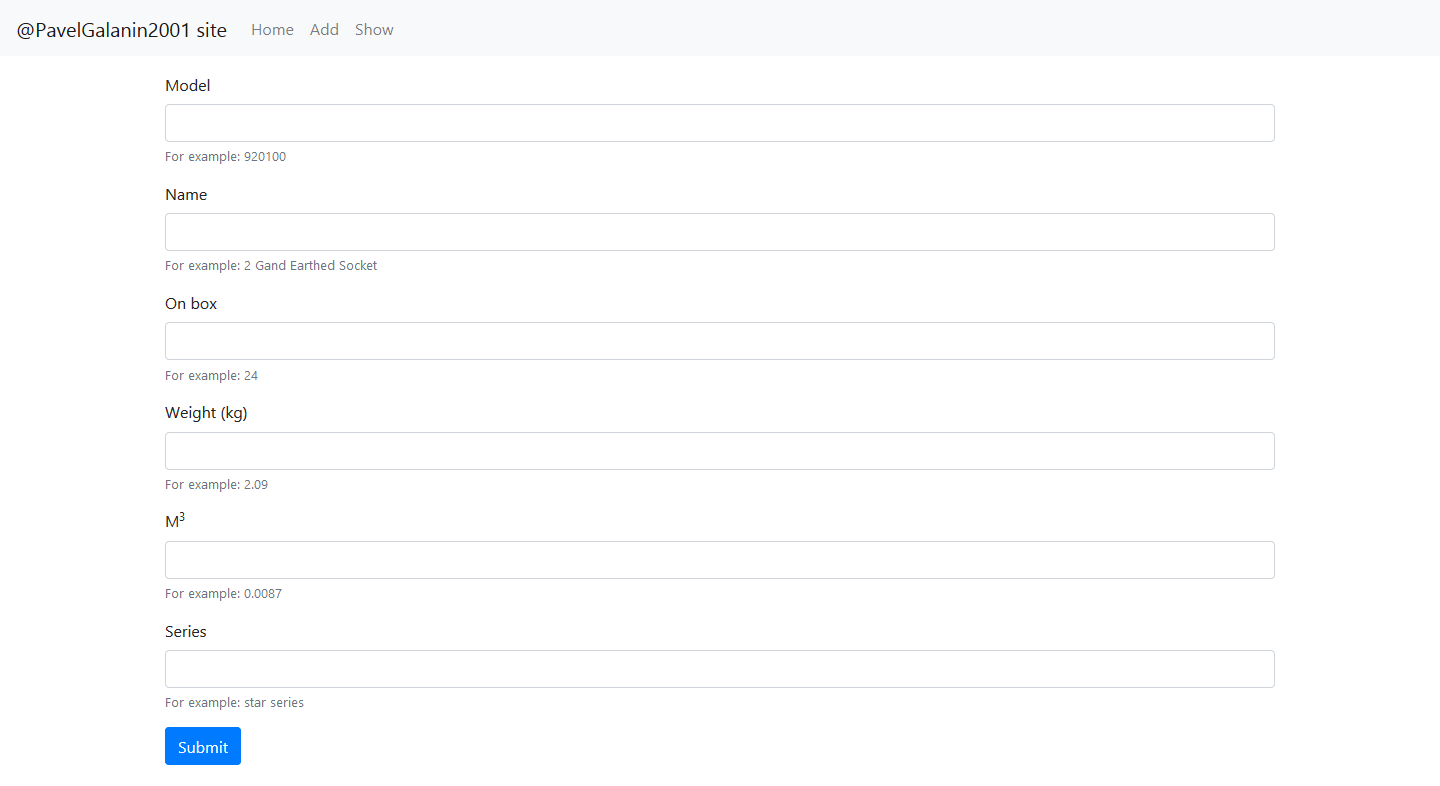
\includegraphics[width=12cm]{../_input/tests/site_form.png}
    \end{center}
    \caption{Форма для добавления элемента\label{fig:site_form}}
\end{figure}

\underline{Полученный результат}:

\begin{itemize}
    \item Таблица MySQL до добавления элемента
    на рисунке \ref{fig:mysql_table_before}
    (стр. \pageref{fig:mysql_table_before}).

    \item Вывод таблицы на сайте до добавления элемента
    на рисунке \ref{fig:site_table_before}
    (стр. \pageref{fig:site_table_before}).

    \item Форма на сайте с заполеными полями
    на рисунке \ref{fig:site_form_add_element_to_table}
    (стр. \pageref{fig:site_form_add_element_to_table}).

    \item Таблица MySQL после добавления элемента
    на рисунке \ref{fig:mysql_table_after}
    (стр. \pageref{fig:mysql_table_after}).

    \item Вывод таблицы на сайте после добавления элемента
    на рисунке \ref{fig:site_table_after}
    (стр. \pageref{fig:site_table_after}).
\end{itemize}

\begin{figure}[!htp]
    \begin{center}
        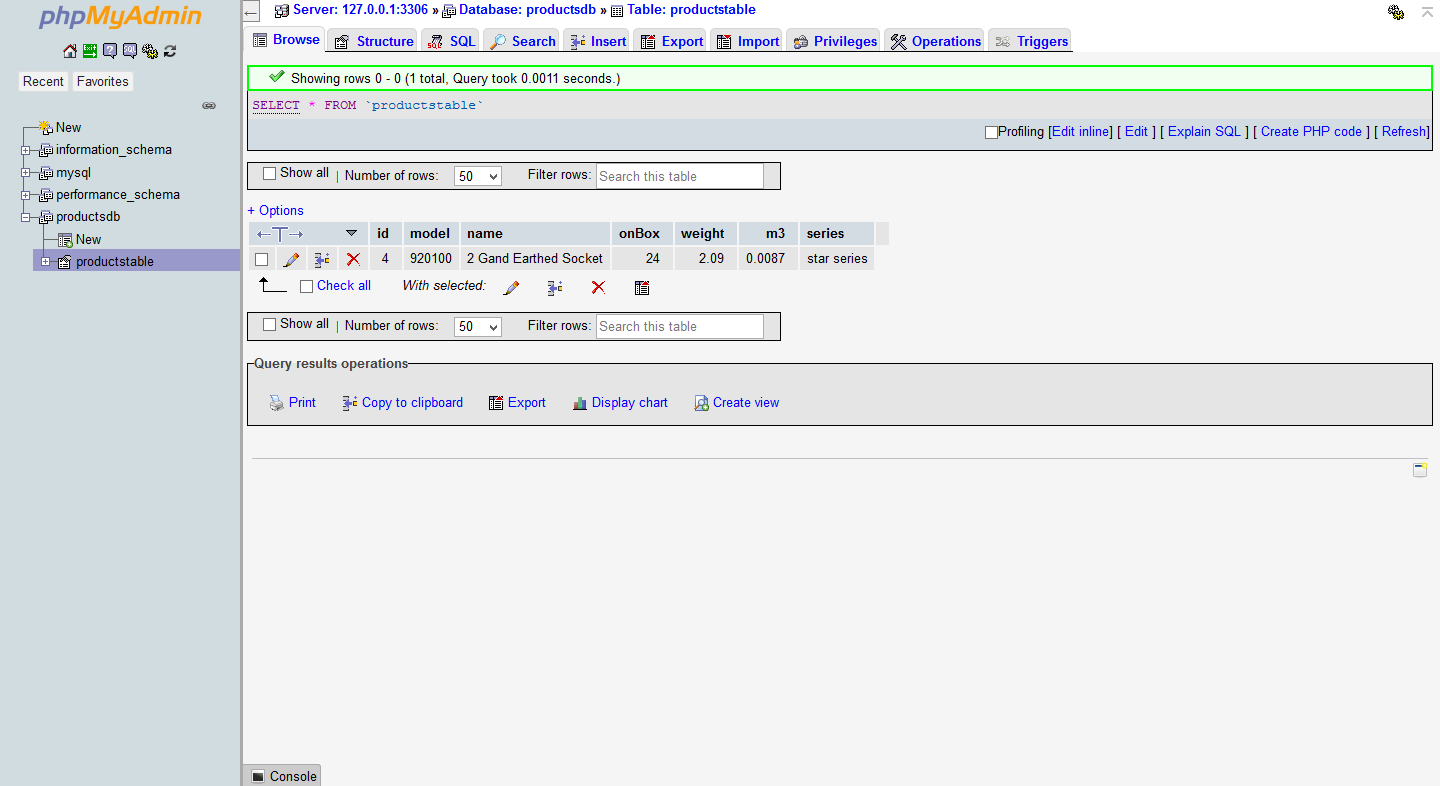
\includegraphics[width=12cm]{../_input/tests/mysql_table_before.png}
    \end{center}
    \caption{Таблица MySQL до добавления элемента\label{fig:mysql_table_before}}
\end{figure}

\begin{figure}[!htp]
    \begin{center}
        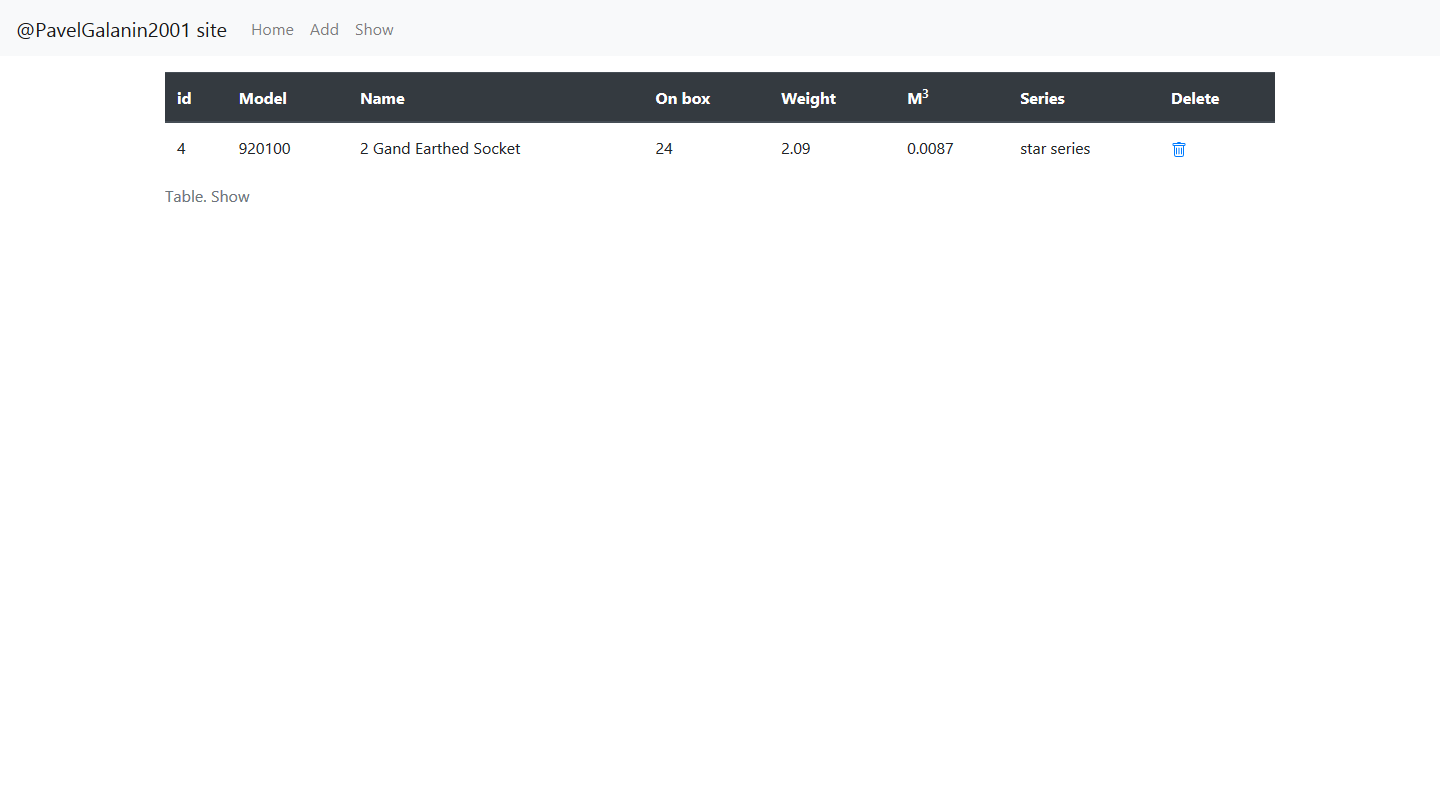
\includegraphics[width=12cm]{../_input/tests/site_table_before.png}
    \end{center}
    \caption{Вывод таблицы на сайте до добавления элемента\label{fig:site_table_before}}
\end{figure}

\begin{figure}[!htp]
    \begin{center}
        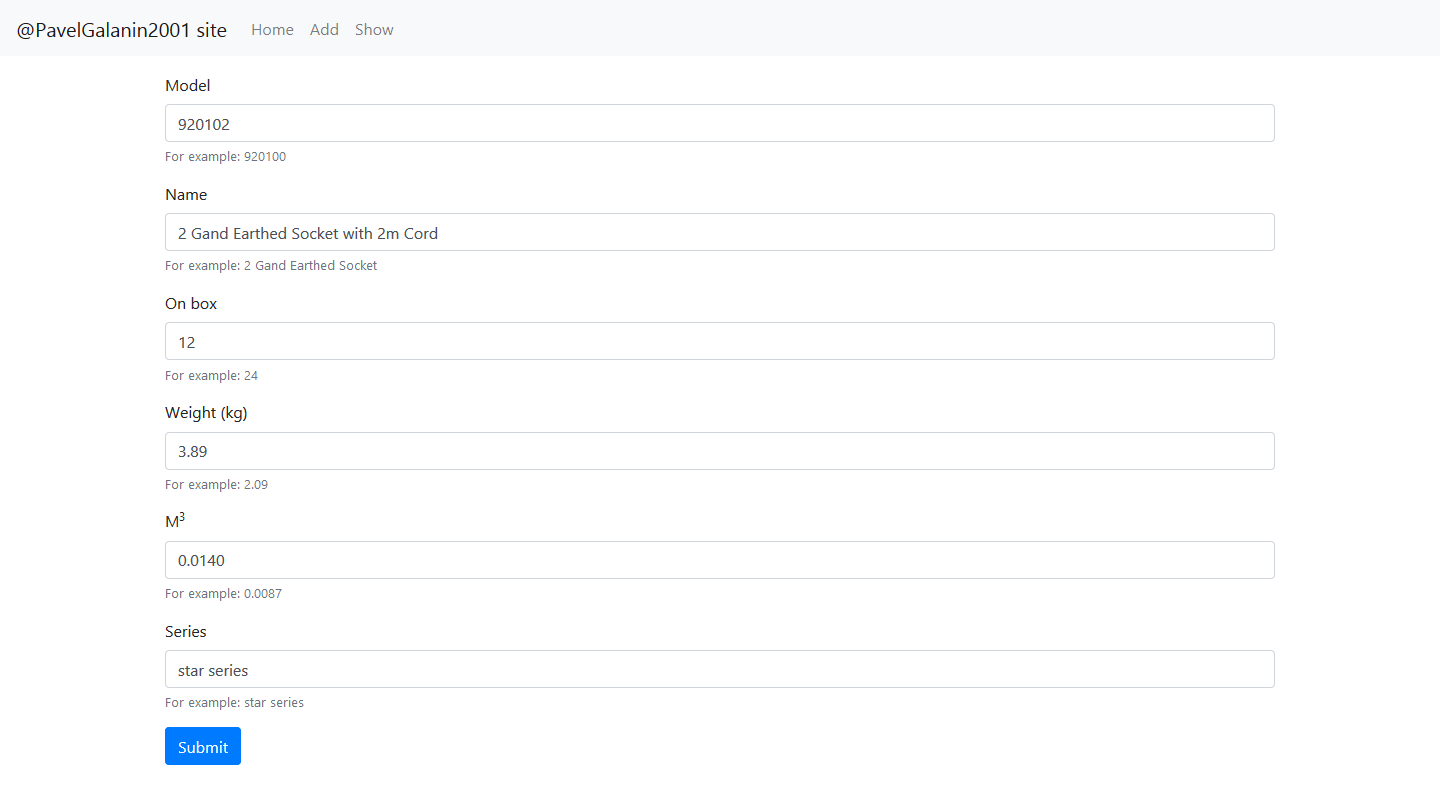
\includegraphics[width=12cm]{../_input/tests/site_form_add_element_to_table.png}
    \end{center}
    \caption{Форма на сайте с заполеными полями\label{fig:site_form_add_element_to_table}}
\end{figure}


\begin{figure}[!htp]
    \begin{center}
        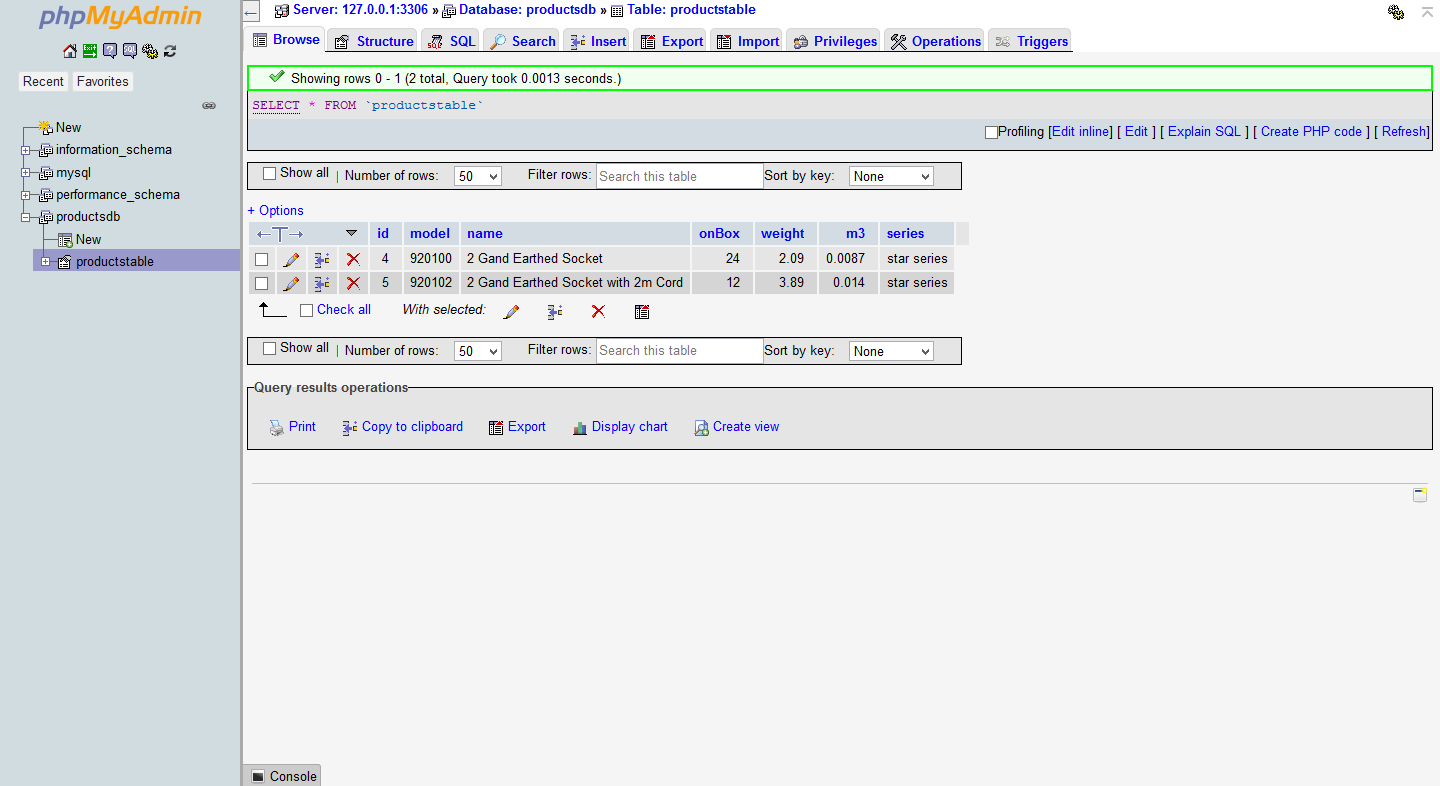
\includegraphics[width=12cm]{../_input/tests/mysql_table_after.png}
    \end{center}
    \caption{Таблица MySQL после добавления элемента\label{fig:mysql_table_after}}
\end{figure}

\begin{figure}[!htp]
    \begin{center}
        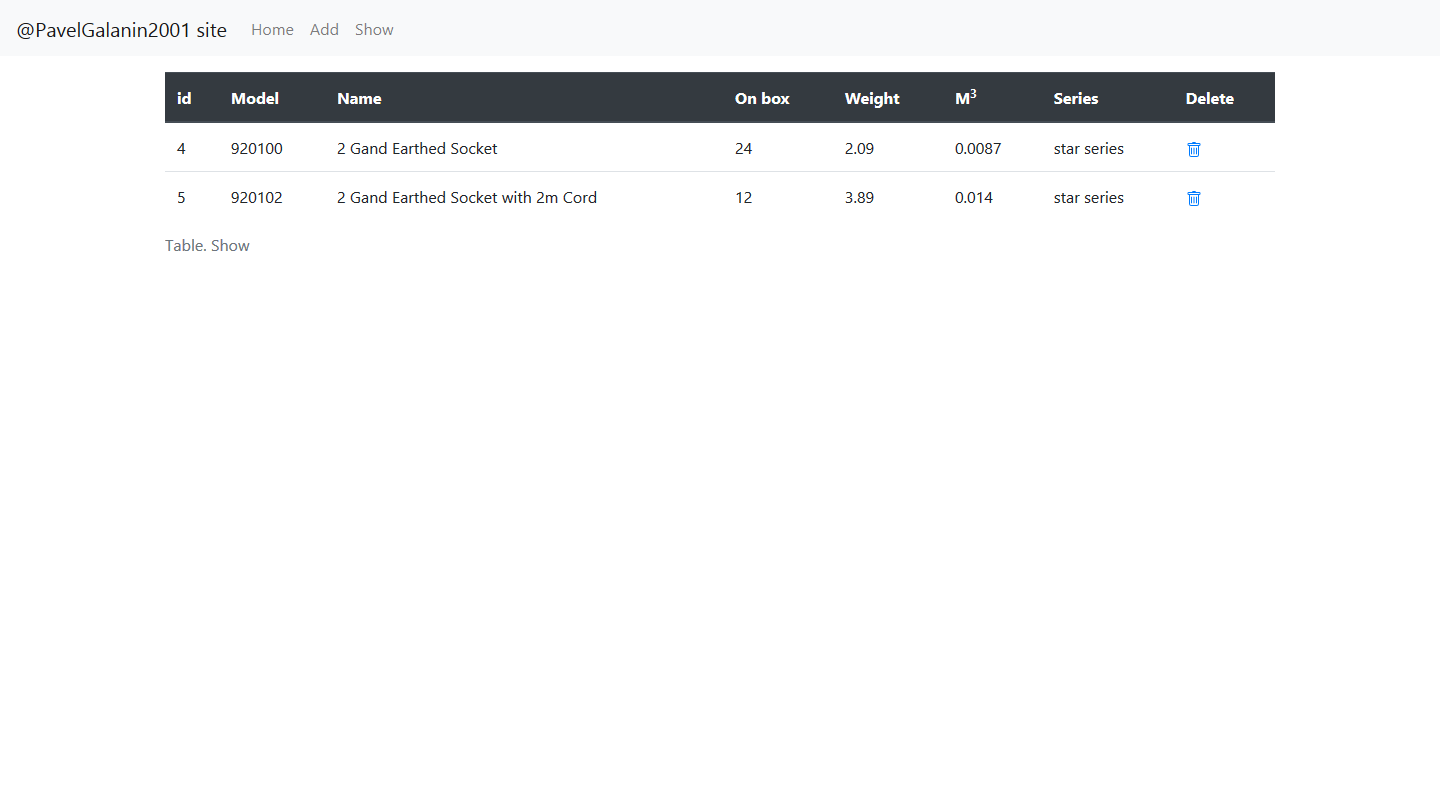
\includegraphics[width=12cm]{../_input/tests/site_table_after.png}
    \end{center}
    \caption{Вывод таблицы на сайте после добавления элемента\label{fig:site_table_after}}
\end{figure}

\underline{Вывод}:
Добавление полей в таблицу MySQL через форму на сайте работает корректно. Поля добавились в таблицу под определённым ID. Ожидаемый результат совпал с полученым.
